\documentclass{standalone}
\usepackage{ProfLycee}
\useproflyclib{ecritures}
\usepackage{tikz}
\begin{document}
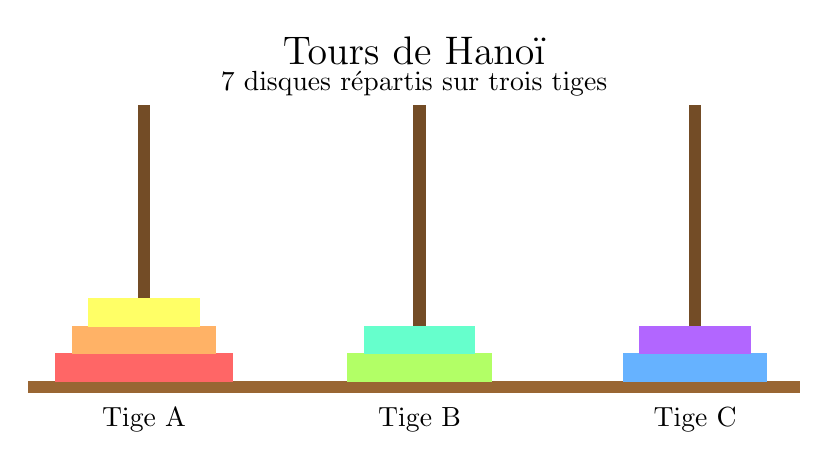
\begin{tikzpicture}[scale=0.7]
  % Définir des couleurs pour les disques
  \definecolor{disk1}{RGB}{255, 102, 102}  % Rouge clair
  \definecolor{disk2}{RGB}{255, 178, 102}  % Orange
  \definecolor{disk3}{RGB}{255, 255, 102}  % Jaune
  \definecolor{disk4}{RGB}{178, 255, 102}  % Vert clair
  \definecolor{disk5}{RGB}{102, 255, 204}  % Turquoise
  \definecolor{disk6}{RGB}{102, 178, 255}  % Bleu clair
  \definecolor{disk7}{RGB}{178, 102, 255}  % Violet

  % Base 
  \filldraw[brown!80!black] (-7,-0.2) rectangle (7,0);
  
  % Tiges
  \filldraw[brown!60!black] (-5,0) rectangle (-4.8,5);
  \filldraw[brown!60!black] (0,0) rectangle (0.2,5);
  \filldraw[brown!60!black] (5,0) rectangle (5.2,5);
  
  % Étiquettes
  \node at (-4.9,-0.7) {Tige A};
  \node at (0.1,-0.7) {Tige B};
  \node at (5.1,-0.7) {Tige C};
  
  % Disques sur la tige A (3 disques)
  \filldraw[disk1] (-6.5,0) rectangle (-3.3,0.5);
  \filldraw[disk2] (-6.2,0.5) rectangle (-3.6,1);
  \filldraw[disk3] (-5.9,1) rectangle (-3.9,1.5);
  
  % Disques sur la tige B (2 disques)
  \filldraw[disk4] (-1.2,0) rectangle (1.4,0.5);
  \filldraw[disk5] (-0.9,0.5) rectangle (1.1,1);
  
  % Disques sur la tige C (2 disques)
  \filldraw[disk6] (3.8,0) rectangle (6.4,0.5);
  \filldraw[disk7] (4.1,0.5) rectangle (6.1,1);
  
  % Titre
  \node at (0,6) {\Large Tours de Hanoï};
  \node at (0,5.4) {7 disques répartis sur trois tiges};
\end{tikzpicture}

\end{document}



Dans le repère orthonormé ci-dessous, on a représenté quelques termes de trois suites arithmétiques.

Pour chacune d'elle, déterminer le premier terme, la raison ainsi que l'expression de $u_n$ en fonction de $n$.
Donner la valeur de $u_3$ et $u_6$.
\begin{center}

  \begin{tikzpicture}[x=0.5cm,y=0.5cm, %unités
    xmin=0,xmax=12,xgrille=1,xgrilles=1, %axe Ox
    ymin=0,ymax=12,ygrille=1,ygrilles=1] %axe Oy
    \FenetreSimpleTikz%
    <Police=\small>{auto}%
    <Police=\small>{auto} %repère

    \foreach \x in {0,...,10} {
      \draw[fill=CouleurVertForet] (\x, \x+1) circle (2pt);
    }
    \foreach \x in {0,5,10} {
      \draw[fill=red] (\x, 0.2*\x+4) circle (2pt);
    }
    \foreach \x in {0,2,4,6,8,10} {
      \draw[fill=blue] (\x, -0.5*\x+7) circle (2pt);
    }
  \end{tikzpicture}
\end{center}
